\documentclass[../main.tex]{subfiles}
\graphicspath{{\subfix{../images/}}}
\begin{document}

\subsection{Stress}
\begin{frame}
  \frametitle{What is Stress? \ldots}
\begin{columns}[c] % The "c" option specifies centered vertical alignment while the "t" option is used for top vertical alignment
\column{.3\textwidth} % Left column and width
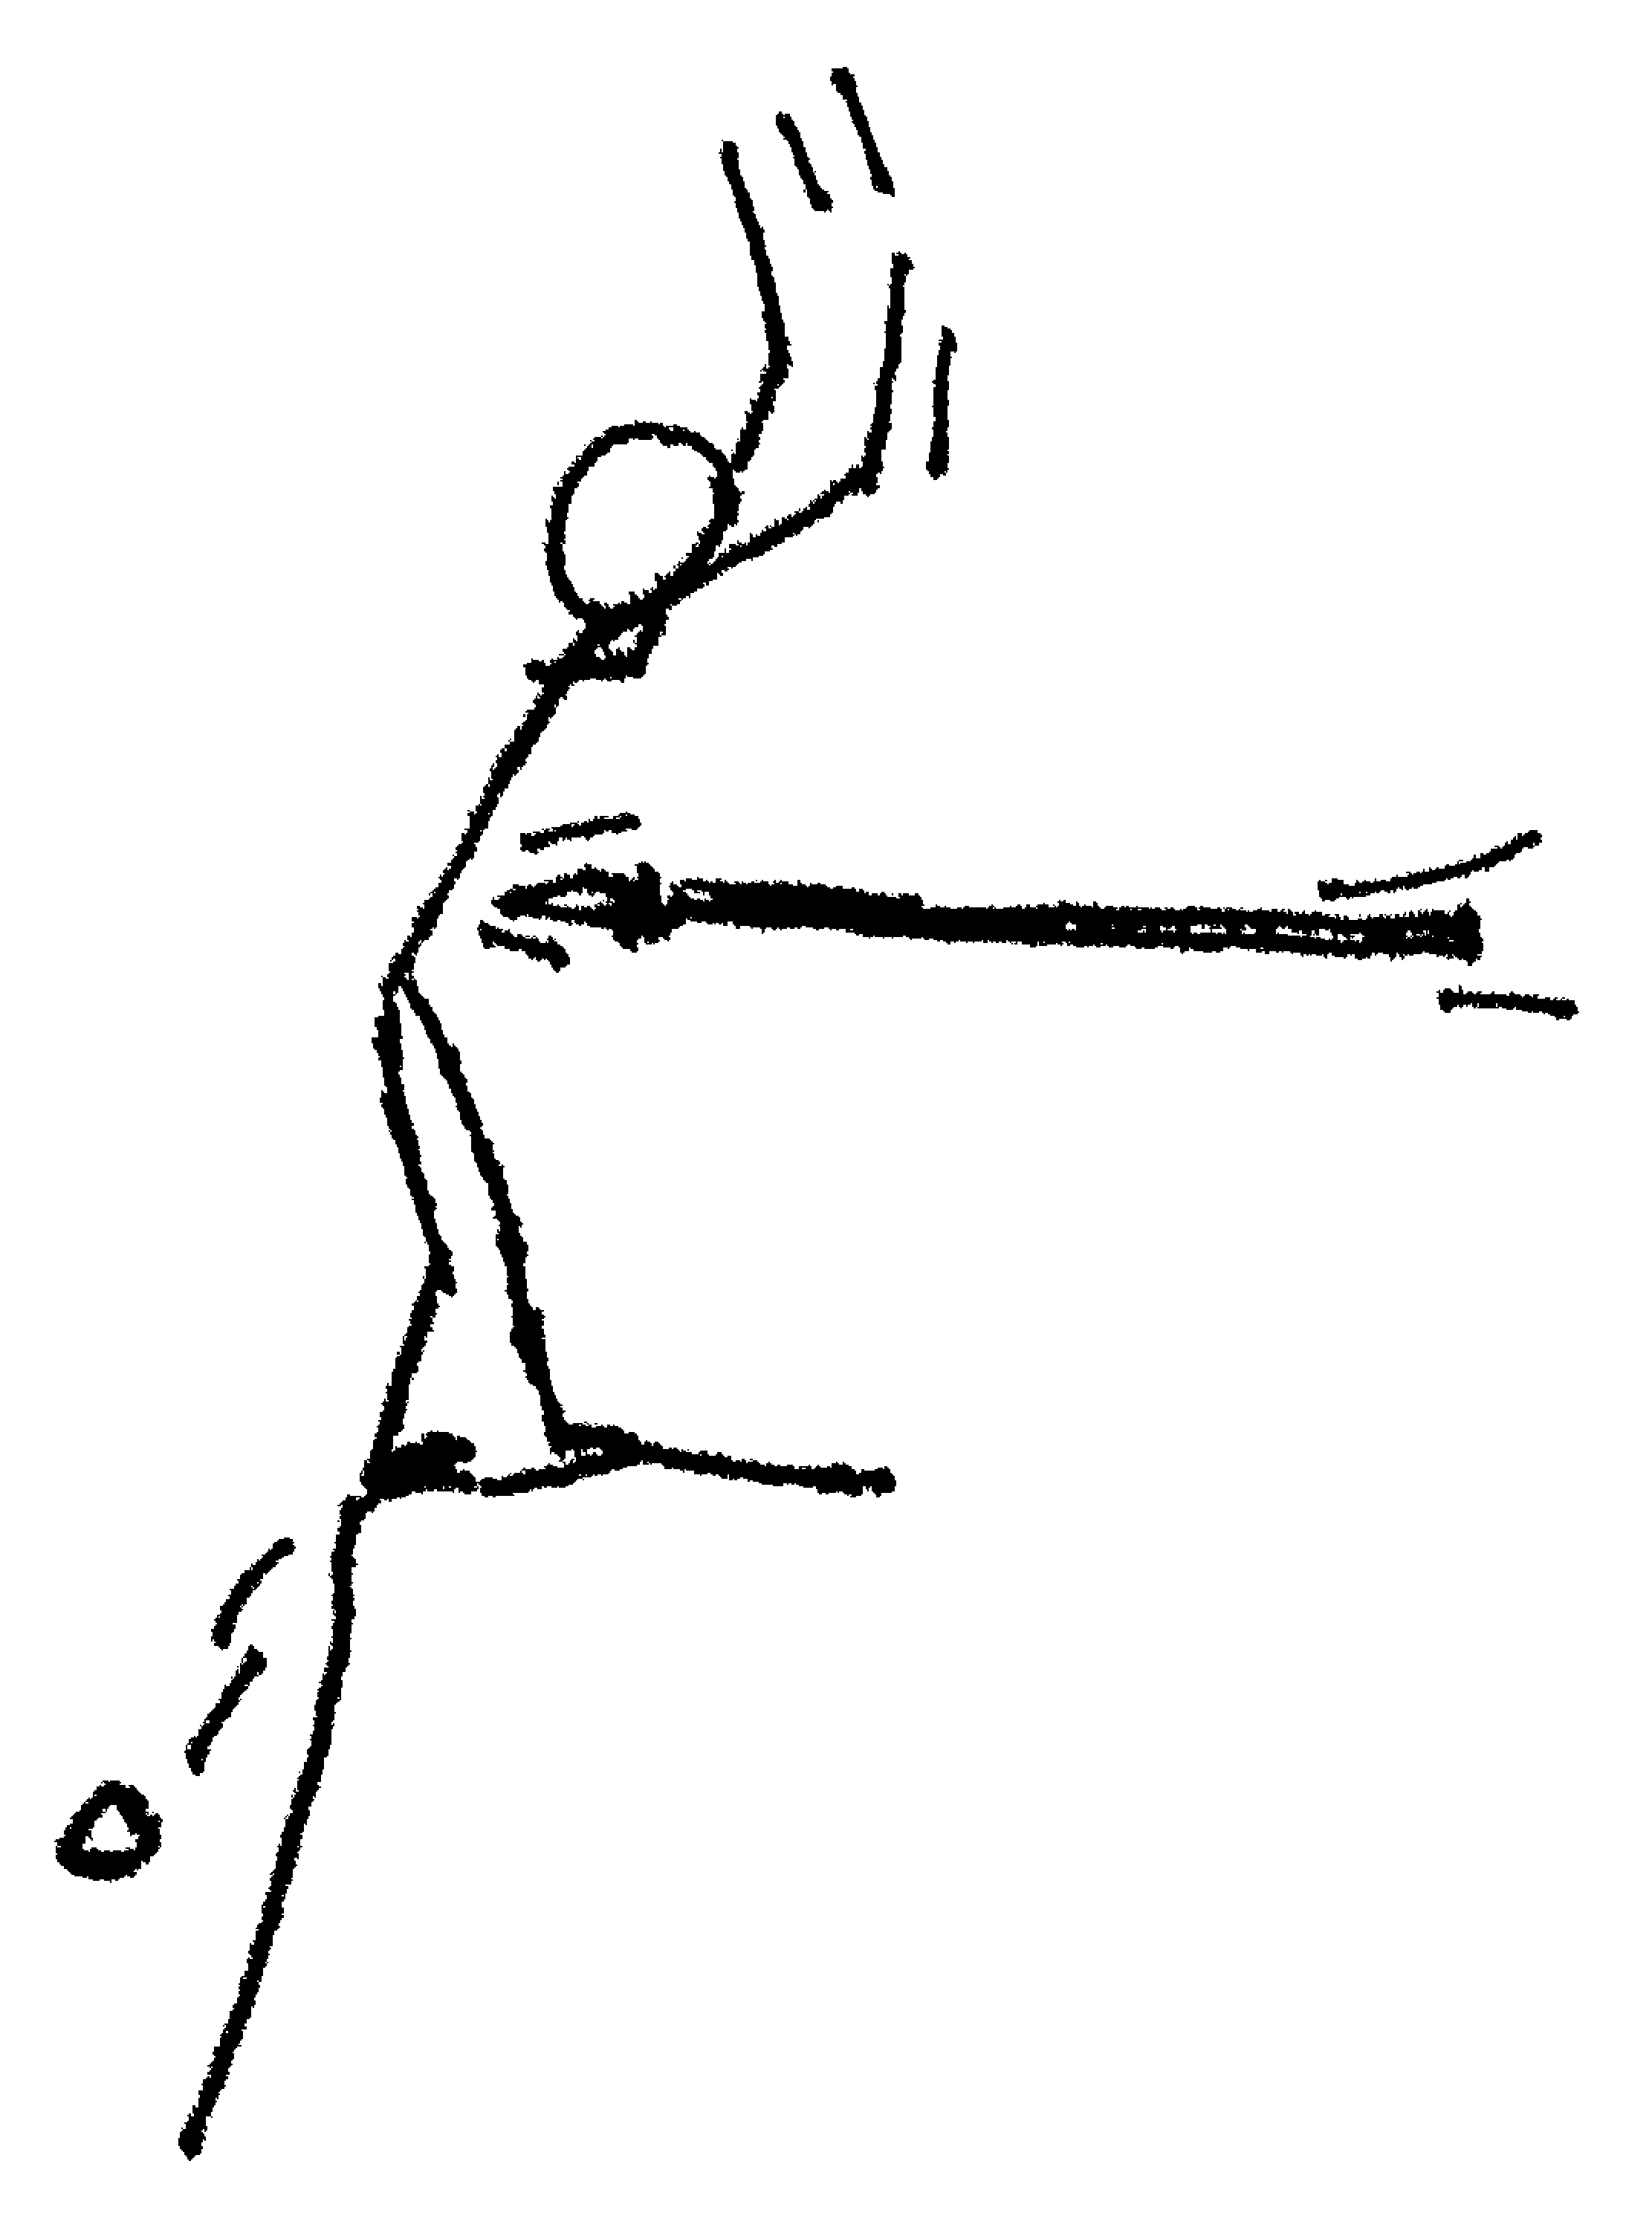
\includegraphics[width=\linewidth]{Guy-Edge}
\column{0.7\textwidth} % Right column and width
is stress in our: \ldots 
 \begin{itemize}
 \item \structure{Outside of us} (yelling person, time pressure, \ldots \structure{stressors})?
 \item  \structure{Body} (muscles, nerves, nervous systems, heart, glands and hormones)?
 \item  \structure{Mind} (fight or flight, coping mechanism, adaptation, mind set)?
   \end{itemize}
\end{columns}
\end{frame}

\begin{frame}
  \frametitle{So where is Stress?}
\begin{columns}[c] % The "c" option specifies centered vertical alignment while the "t" option is used for top vertical alignment
\column{.4\textwidth} % Left column and width
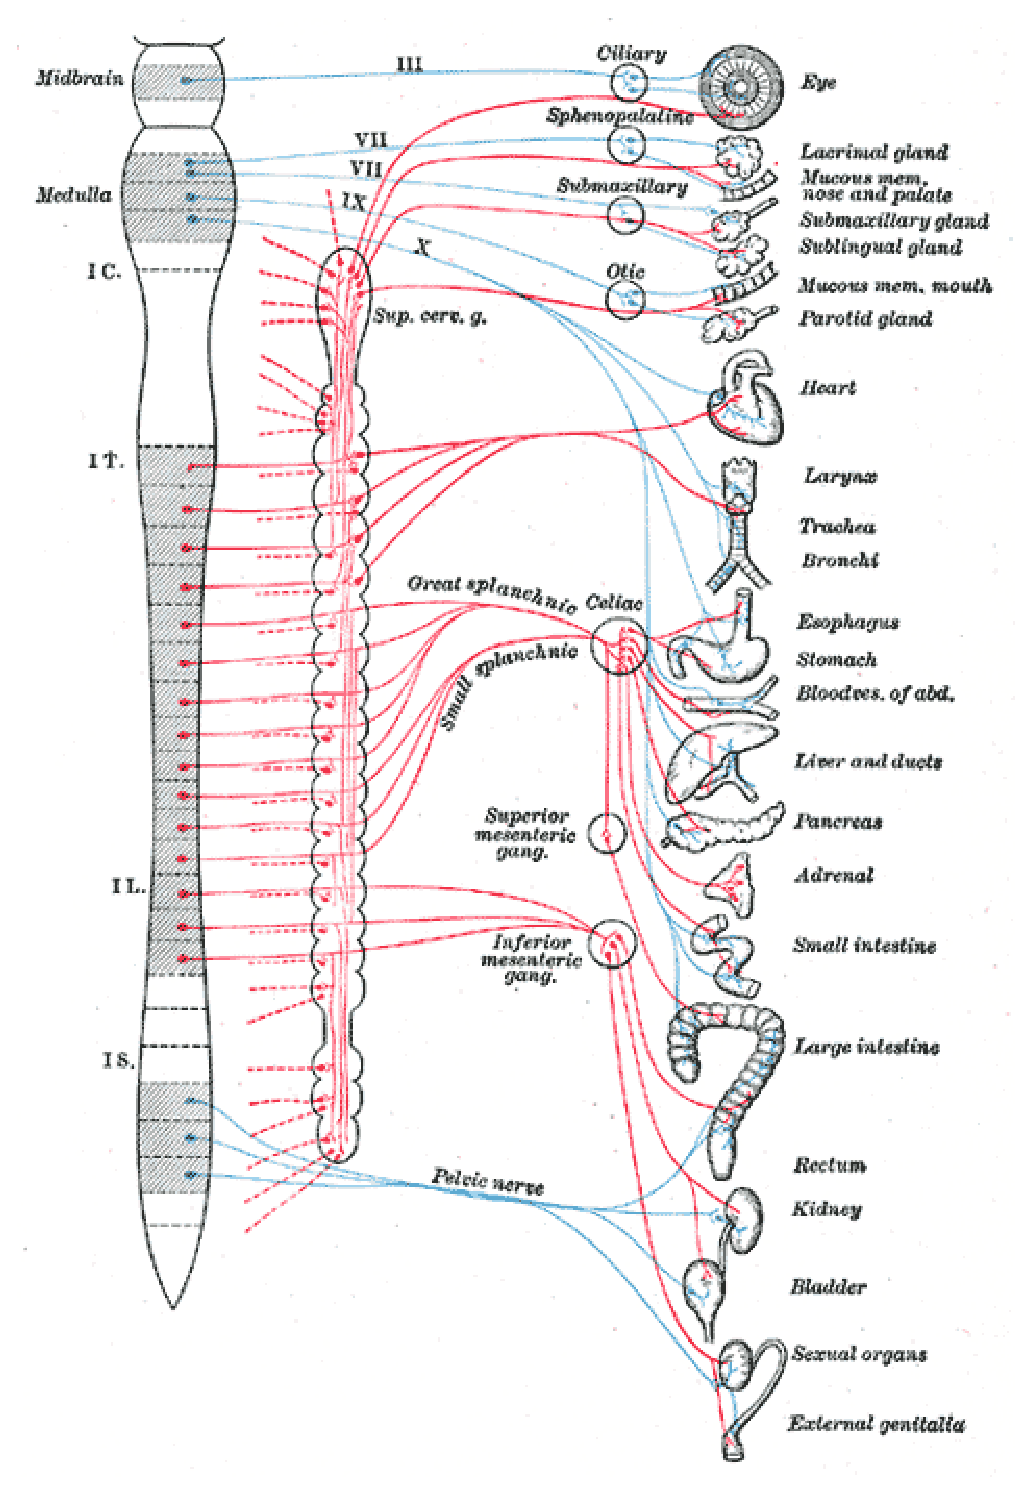
\includegraphics[width=1\linewidth]{AutonomousNS}

\small{The sympathetic nervous system (red).}
\column{0.6\textwidth} % Right column and width
 \begin{itemize}
 \item \structure{Stressors} are perceived by \structure{sensory cells} and the impulse transmitted over the \structure{nervous system}.
 \item  The \alert{limbic system} evaluates threat levels.
 \item  \structure{Fight or flight} might get triggered, stress hormones releases.
 \item The \structure{sympathetic nervous system} activated, which readies the body for survival.
   \end{itemize}
\end{columns}
\end{frame}

\subsection{The limbic system}

\begin{frame}
  \frametitle{What is the limbic system?}
  The limbic system regulates the stress reaction (fight or flight). It gives different signals different meanings (ignore, stress).
  It regulates next to stress:

\vspace{5mm}
  \begin{columns}[c] % The "c" option specifies centered vertical alignment while the "t" option is used for top vertical alignment
\column{.6\textwidth} % Left column and width
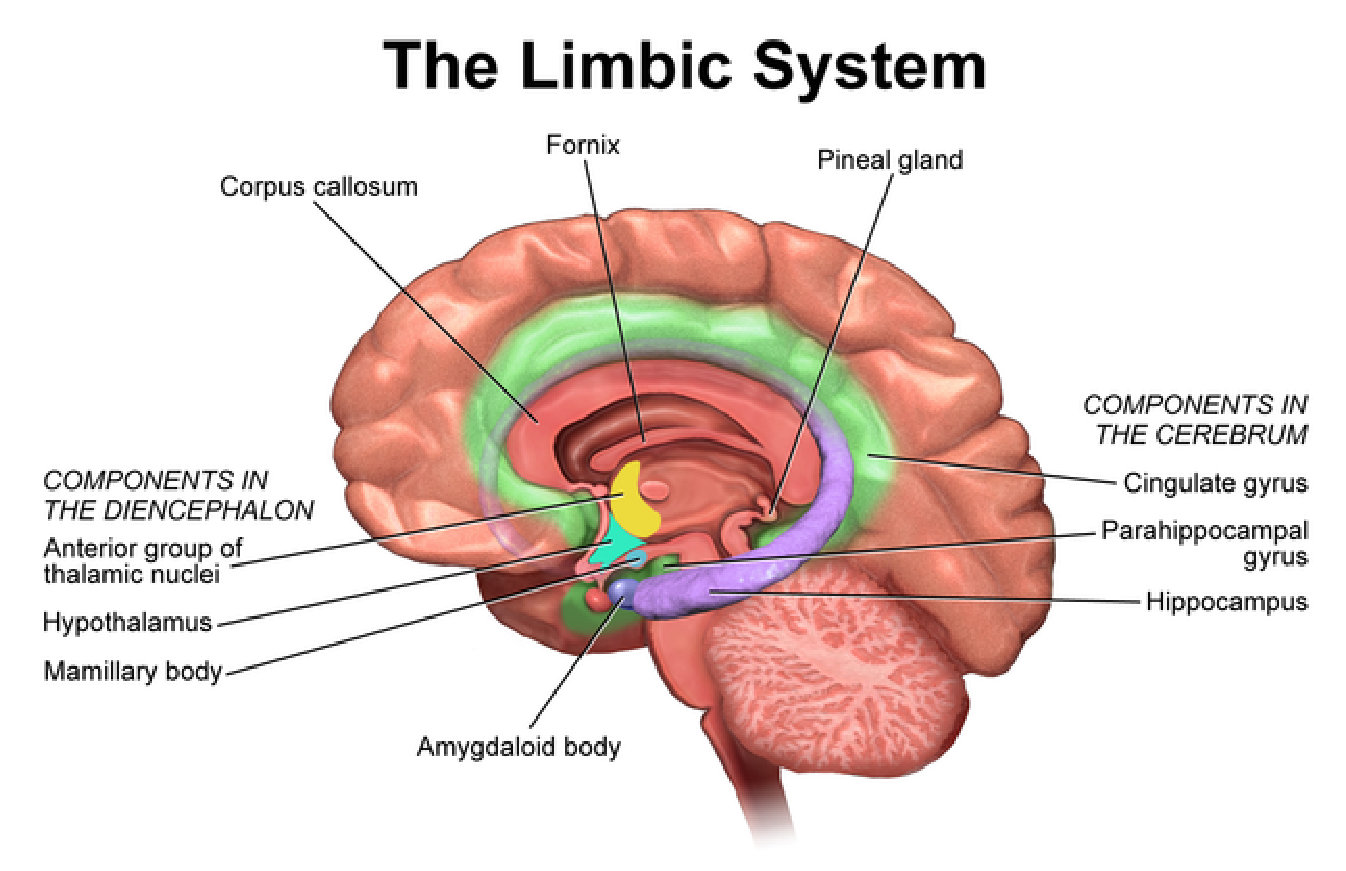
\includegraphics[width=\linewidth]{LimbicSystem}
\column{0.4\textwidth} % Right column and width

  \begin{itemize}
  \item - Emotions
  \item - Sleep/awake state
  \item - Nutrition
  \item - and procreation
  \end{itemize}

\end{columns}

\end{frame}

\subsection{Stress regulation}

\begin{frame}
\frametitle{Stress is unavoidable in life, \ldots}
\begin{columns}[c] % The "c" option specifies centered vertical alignment while the "t" option is used for top vertical alignment
\column{.3\textwidth} % Left column and width
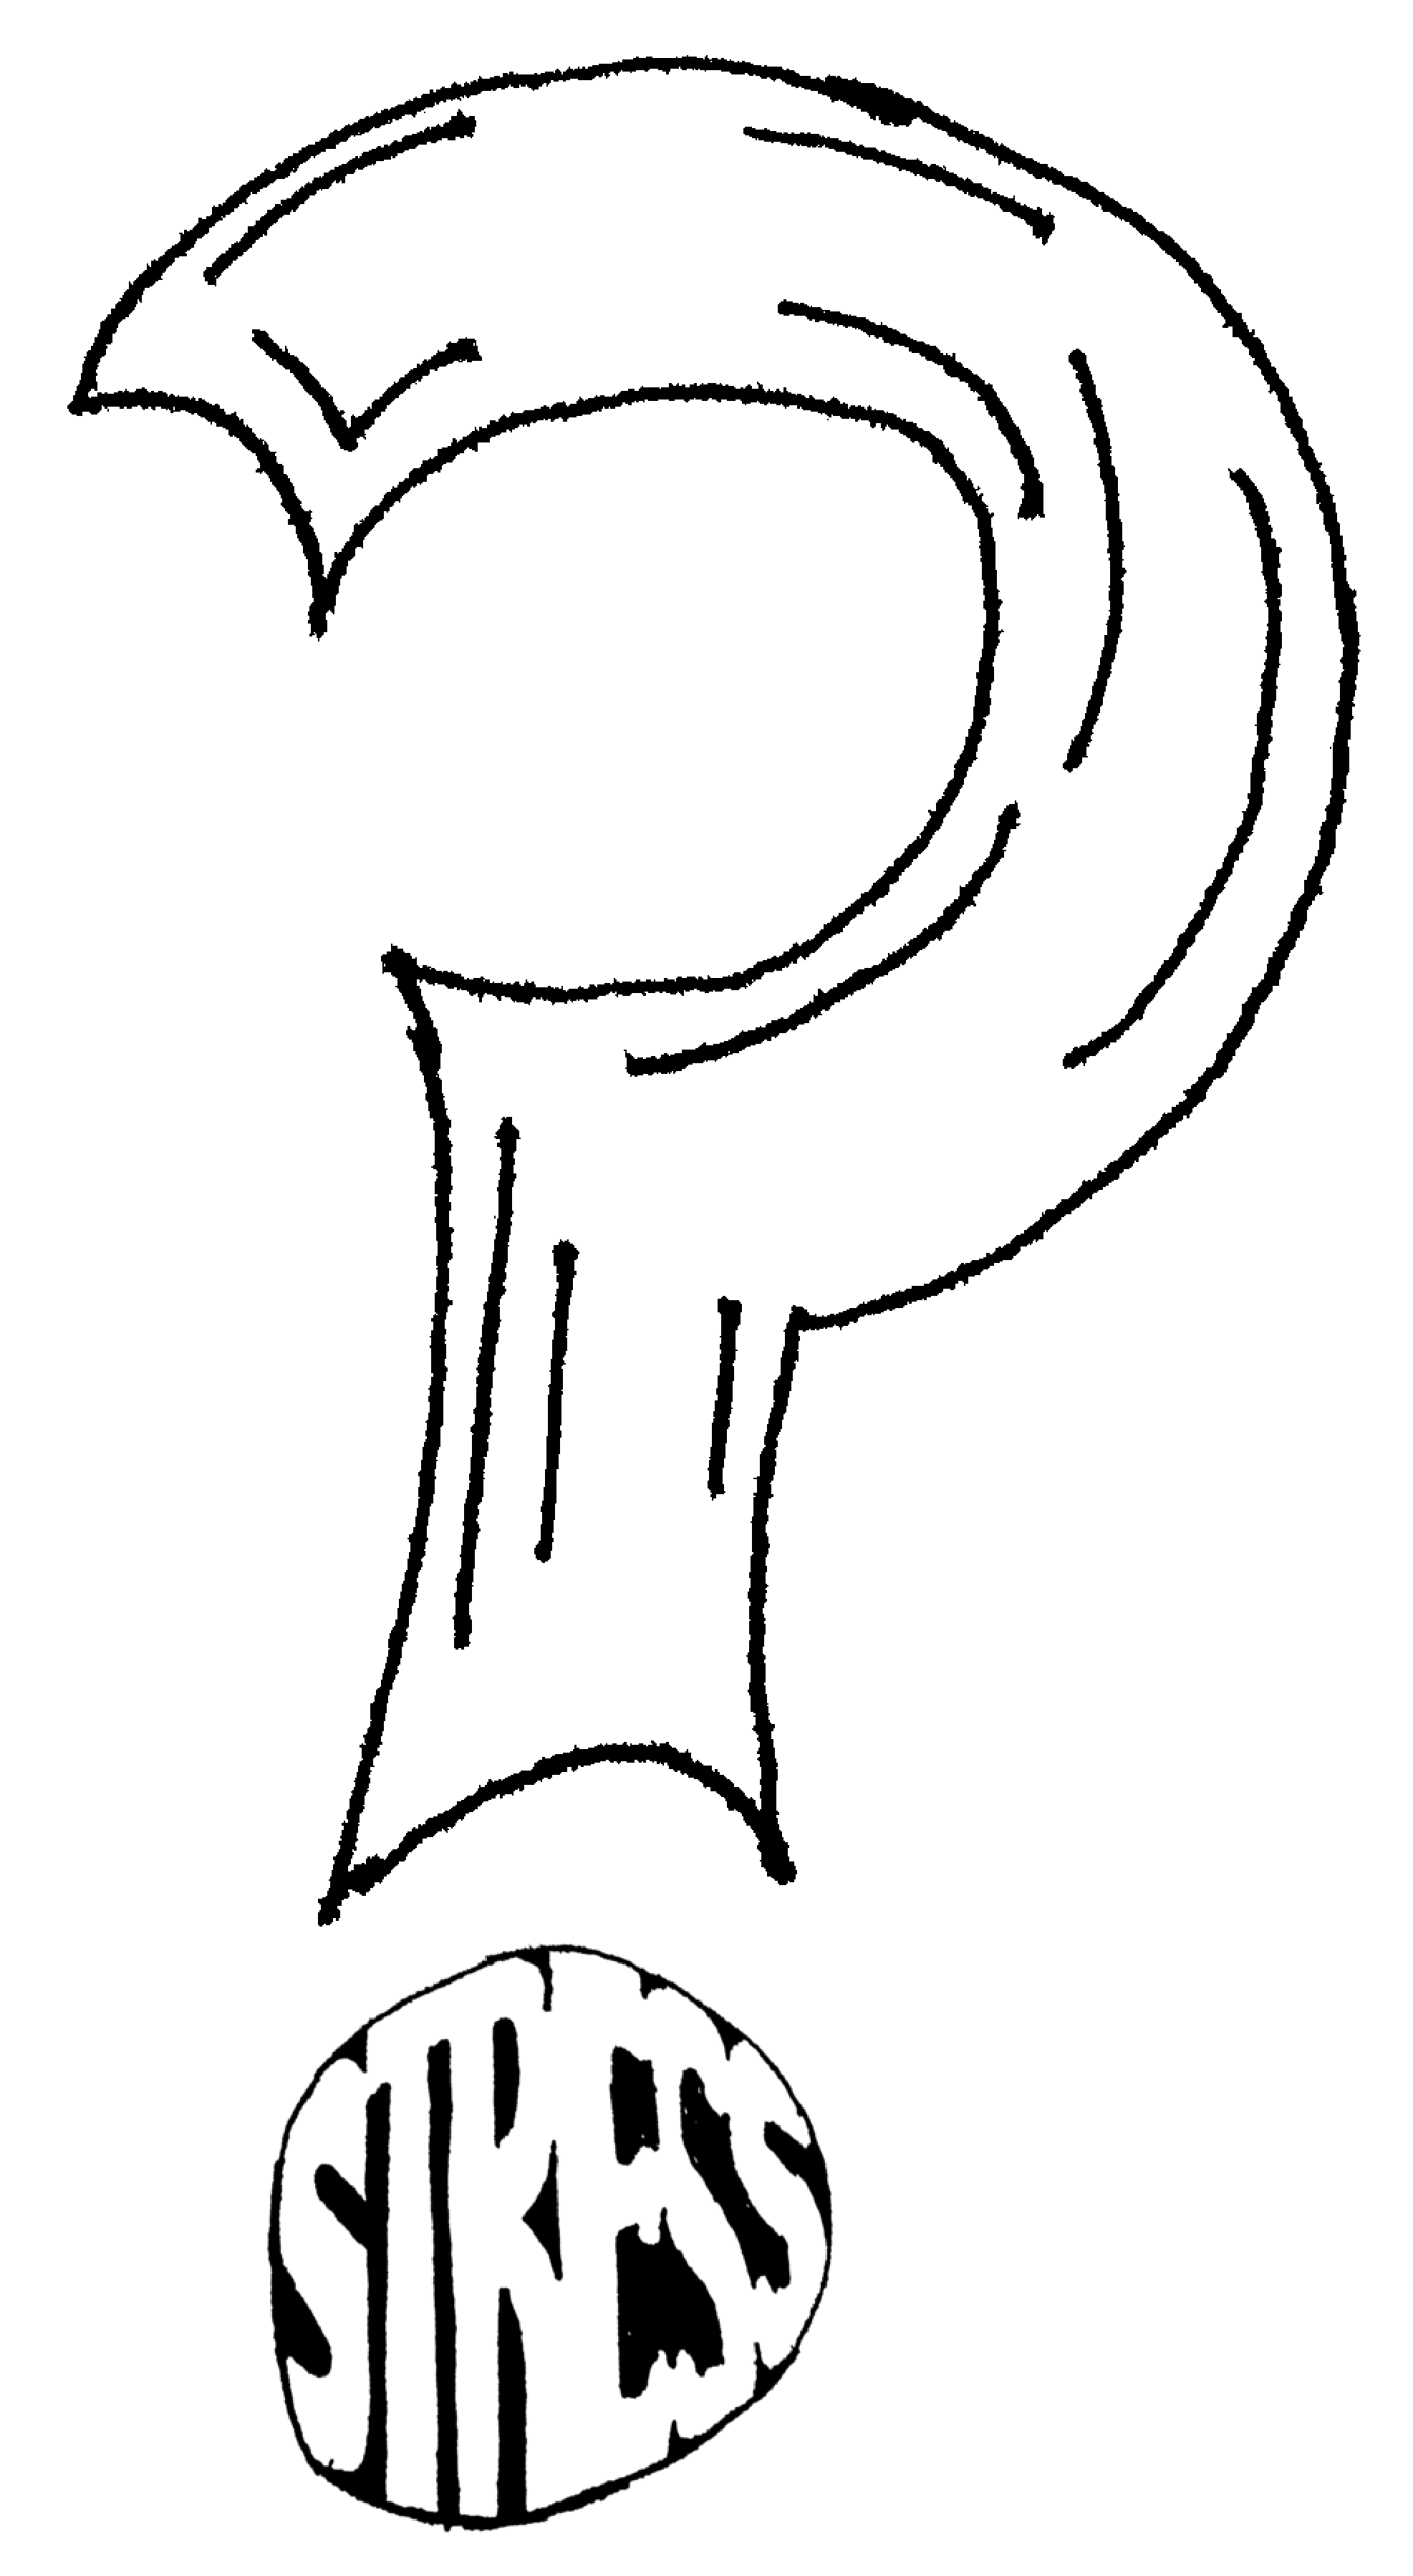
\includegraphics[width=\linewidth]{Question}
\column{0.7\textwidth} % Right column and width
 but can we do something? \ldots 
 \begin{itemize}
 \item \structure{Regulate}
 \item \structure{Negative stress} vs \structure{positive stress}
 \item \structure{Stress resistance} 
 \item \structure{Relaxation} and \structure{mindfulness} exercises
 \item \structure{Eat consciously}
 \item A \structure{mindful life} 
 \end{itemize}
\end{columns}
\end{frame}



\end{document}